% Options for packages loaded elsewhere
\PassOptionsToPackage{unicode}{hyperref}
\PassOptionsToPackage{hyphens}{url}
%
\documentclass[
  ignorenonframetext,
]{beamer}
\usepackage{pgfpages}
\setbeamertemplate{caption}[numbered]
\setbeamertemplate{caption label separator}{: }
\setbeamercolor{caption name}{fg=normal text.fg}
\beamertemplatenavigationsymbolsempty
% Prevent slide breaks in the middle of a paragraph
\widowpenalties 1 10000
\raggedbottom
\setbeamertemplate{part page}{
  \centering
  \begin{beamercolorbox}[sep=16pt,center]{part title}
    \usebeamerfont{part title}\insertpart\par
  \end{beamercolorbox}
}
\setbeamertemplate{section page}{
  \centering
  \begin{beamercolorbox}[sep=12pt,center]{part title}
    \usebeamerfont{section title}\insertsection\par
  \end{beamercolorbox}
}
\setbeamertemplate{subsection page}{
  \centering
  \begin{beamercolorbox}[sep=8pt,center]{part title}
    \usebeamerfont{subsection title}\insertsubsection\par
  \end{beamercolorbox}
}
\AtBeginPart{
  \frame{\partpage}
}
\AtBeginSection{
  \ifbibliography
  \else
    \frame{\sectionpage}
  \fi
}
\AtBeginSubsection{
  \frame{\subsectionpage}
}
\usepackage{amsmath,amssymb}
\usepackage{iftex}
\ifPDFTeX
  \usepackage[T1]{fontenc}
  \usepackage[utf8]{inputenc}
  \usepackage{textcomp} % provide euro and other symbols
\else % if luatex or xetex
  \usepackage{unicode-math} % this also loads fontspec
  \defaultfontfeatures{Scale=MatchLowercase}
  \defaultfontfeatures[\rmfamily]{Ligatures=TeX,Scale=1}
\fi
\usepackage{lmodern}
\usetheme[]{Madrid}
\ifPDFTeX\else
  % xetex/luatex font selection
\fi
% Use upquote if available, for straight quotes in verbatim environments
\IfFileExists{upquote.sty}{\usepackage{upquote}}{}
\IfFileExists{microtype.sty}{% use microtype if available
  \usepackage[]{microtype}
  \UseMicrotypeSet[protrusion]{basicmath} % disable protrusion for tt fonts
}{}
\makeatletter
\@ifundefined{KOMAClassName}{% if non-KOMA class
  \IfFileExists{parskip.sty}{%
    \usepackage{parskip}
  }{% else
    \setlength{\parindent}{0pt}
    \setlength{\parskip}{6pt plus 2pt minus 1pt}}
}{% if KOMA class
  \KOMAoptions{parskip=half}}
\makeatother
\usepackage{xcolor}
\newif\ifbibliography
\usepackage{color}
\usepackage{fancyvrb}
\newcommand{\VerbBar}{|}
\newcommand{\VERB}{\Verb[commandchars=\\\{\}]}
\DefineVerbatimEnvironment{Highlighting}{Verbatim}{commandchars=\\\{\}}
% Add ',fontsize=\small' for more characters per line
\usepackage{framed}
\definecolor{shadecolor}{RGB}{248,248,248}
\newenvironment{Shaded}{\begin{snugshade}}{\end{snugshade}}
\newcommand{\AlertTok}[1]{\textcolor[rgb]{0.94,0.16,0.16}{#1}}
\newcommand{\AnnotationTok}[1]{\textcolor[rgb]{0.56,0.35,0.01}{\textbf{\textit{#1}}}}
\newcommand{\AttributeTok}[1]{\textcolor[rgb]{0.13,0.29,0.53}{#1}}
\newcommand{\BaseNTok}[1]{\textcolor[rgb]{0.00,0.00,0.81}{#1}}
\newcommand{\BuiltInTok}[1]{#1}
\newcommand{\CharTok}[1]{\textcolor[rgb]{0.31,0.60,0.02}{#1}}
\newcommand{\CommentTok}[1]{\textcolor[rgb]{0.56,0.35,0.01}{\textit{#1}}}
\newcommand{\CommentVarTok}[1]{\textcolor[rgb]{0.56,0.35,0.01}{\textbf{\textit{#1}}}}
\newcommand{\ConstantTok}[1]{\textcolor[rgb]{0.56,0.35,0.01}{#1}}
\newcommand{\ControlFlowTok}[1]{\textcolor[rgb]{0.13,0.29,0.53}{\textbf{#1}}}
\newcommand{\DataTypeTok}[1]{\textcolor[rgb]{0.13,0.29,0.53}{#1}}
\newcommand{\DecValTok}[1]{\textcolor[rgb]{0.00,0.00,0.81}{#1}}
\newcommand{\DocumentationTok}[1]{\textcolor[rgb]{0.56,0.35,0.01}{\textbf{\textit{#1}}}}
\newcommand{\ErrorTok}[1]{\textcolor[rgb]{0.64,0.00,0.00}{\textbf{#1}}}
\newcommand{\ExtensionTok}[1]{#1}
\newcommand{\FloatTok}[1]{\textcolor[rgb]{0.00,0.00,0.81}{#1}}
\newcommand{\FunctionTok}[1]{\textcolor[rgb]{0.13,0.29,0.53}{\textbf{#1}}}
\newcommand{\ImportTok}[1]{#1}
\newcommand{\InformationTok}[1]{\textcolor[rgb]{0.56,0.35,0.01}{\textbf{\textit{#1}}}}
\newcommand{\KeywordTok}[1]{\textcolor[rgb]{0.13,0.29,0.53}{\textbf{#1}}}
\newcommand{\NormalTok}[1]{#1}
\newcommand{\OperatorTok}[1]{\textcolor[rgb]{0.81,0.36,0.00}{\textbf{#1}}}
\newcommand{\OtherTok}[1]{\textcolor[rgb]{0.56,0.35,0.01}{#1}}
\newcommand{\PreprocessorTok}[1]{\textcolor[rgb]{0.56,0.35,0.01}{\textit{#1}}}
\newcommand{\RegionMarkerTok}[1]{#1}
\newcommand{\SpecialCharTok}[1]{\textcolor[rgb]{0.81,0.36,0.00}{\textbf{#1}}}
\newcommand{\SpecialStringTok}[1]{\textcolor[rgb]{0.31,0.60,0.02}{#1}}
\newcommand{\StringTok}[1]{\textcolor[rgb]{0.31,0.60,0.02}{#1}}
\newcommand{\VariableTok}[1]{\textcolor[rgb]{0.00,0.00,0.00}{#1}}
\newcommand{\VerbatimStringTok}[1]{\textcolor[rgb]{0.31,0.60,0.02}{#1}}
\newcommand{\WarningTok}[1]{\textcolor[rgb]{0.56,0.35,0.01}{\textbf{\textit{#1}}}}
\usepackage{graphicx}
\makeatletter
\def\maxwidth{\ifdim\Gin@nat@width>\linewidth\linewidth\else\Gin@nat@width\fi}
\def\maxheight{\ifdim\Gin@nat@height>\textheight\textheight\else\Gin@nat@height\fi}
\makeatother
% Scale images if necessary, so that they will not overflow the page
% margins by default, and it is still possible to overwrite the defaults
% using explicit options in \includegraphics[width, height, ...]{}
\setkeys{Gin}{width=\maxwidth,height=\maxheight,keepaspectratio}
% Set default figure placement to htbp
\makeatletter
\def\fps@figure{htbp}
\makeatother
\setlength{\emergencystretch}{3em} % prevent overfull lines
\providecommand{\tightlist}{%
  \setlength{\itemsep}{0pt}\setlength{\parskip}{0pt}}
\setcounter{secnumdepth}{-\maxdimen} % remove section numbering
\logo{
\includegraphics[height=1cm,width=3cm]{logo.png}}
\usetheme{Madrid}
\usefonttheme{serif}
\setbeamertemplate{navigation symbols}{}
\usepackage{lmodern}  % for bold teletype font
\usepackage{amsmath}  % for \hookrightarrow
\usepackage{xcolor}   % for \textcolor


\ifLuaTeX
  \usepackage{selnolig}  % disable illegal ligatures
\fi
\usepackage{bookmark}
\IfFileExists{xurl.sty}{\usepackage{xurl}}{} % add URL line breaks if available
\urlstyle{same}
\hypersetup{
  pdftitle={Leksioni 11},
  pdfauthor={Endri Raco},
  hidelinks,
  pdfcreator={LaTeX via pandoc}}

\title{Leksioni 11}
\author{Endri Raco}
\date{02 July, 2024}

\begin{document}
\frame{\titlepage}

\begin{frame}[allowframebreaks]
  \tableofcontents[hideallsubsections]
\end{frame}
\section{Hyrje në SQL}\label{hyrje-nuxeb-sql}

\begin{frame}{Si të shkarkoni SQL Server Setup}
\phantomsection\label{si-tuxeb-shkarkoni-sql-server-setup}
\textbf{Hapi 1} Shkoni te URL-ja:
\url{https://www.microsoft.com/en-in/sql-server/sql-server-downloads}
për shkarkim të serverit Microsoft SQL.
\end{frame}

\begin{frame}{Si të shkarkoni SQL Server Setup}
\phantomsection\label{si-tuxeb-shkarkoni-sql-server-setup-1}
Microsoft ofron dy edicione të specializuara të shkarkimit falas të SQL
për të punuar në MS SQL Server:

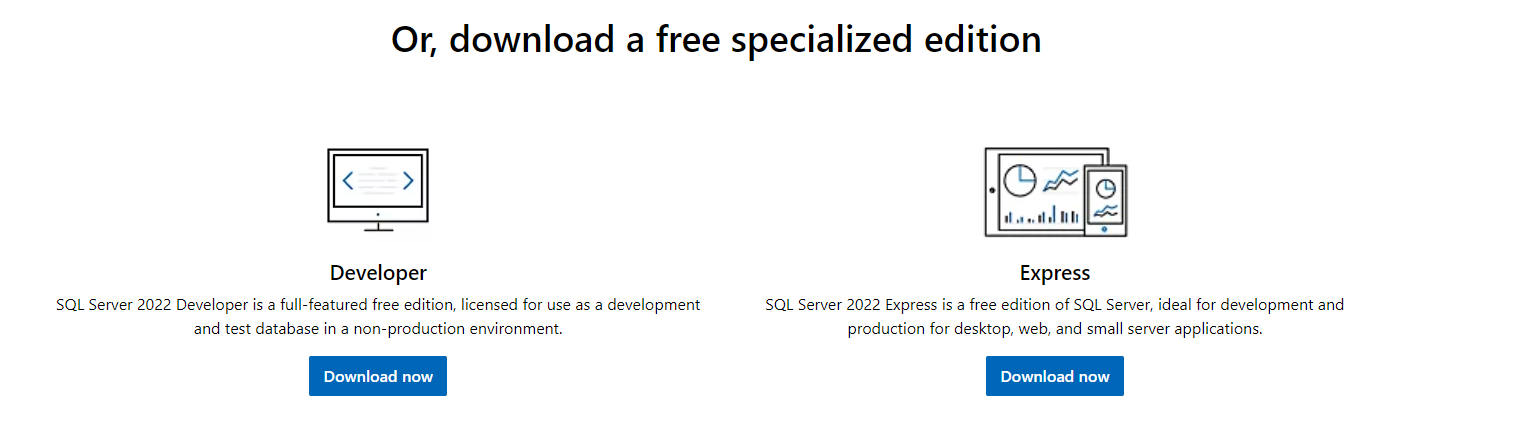
\includegraphics{./Figs/install1.png}
\end{frame}

\begin{frame}{Si të shkarkoni SQL Server Setup}
\phantomsection\label{si-tuxeb-shkarkoni-sql-server-setup-2}
\textbf{Developer} -- Ka të gjitha veçoritë që ofron MS SQL Server, por
nuk mund ta përdorim atë në prodhim.

Nga këndvështrimi i të mësuarit, a është një kandidat ideal për të
filluar.
\end{frame}

\begin{frame}{Si të shkarkoni SQL Server Setup}
\phantomsection\label{si-tuxeb-shkarkoni-sql-server-setup-3}
\textbf{Express}: Ky është gjithashtu një version falas i MS SQL Server,
por me disa kufizime në aplikimet e inteligjencës së biznesit.
\end{frame}

\begin{frame}{Si të shkarkoni SQL Server Setup}
\phantomsection\label{si-tuxeb-shkarkoni-sql-server-setup-4}
Ne do të zgjedhim versionin Developer për të shkarkuar serverin
Microsoft SQL për instalim.

\textbf{Hapi 2} Klikoni në ``Download Now''

Shkarkoni SQL Server Setup
\end{frame}

\begin{frame}{Si të shkarkoni SQL Server Setup}
\phantomsection\label{si-tuxeb-shkarkoni-sql-server-setup-5}
Ne do të marrim instalimin e serverit SQL të konfiguruar si
`SQLServer2022SSEI-Dev.exe' në një mjedis Windows, duke siguruar
përputhshmëri dhe performancë të optimizuar për aplikacionet SQL Server
Windows.
\end{frame}

\begin{frame}{Si të instaloni Microsoft SQL Server}
\phantomsection\label{si-tuxeb-instaloni-microsoft-sql-server}
Këtu është një proces hap pas hapi se si të instaloni SQL në Windows 10:

\textbf{Hapi 1} Hapni skedarin \textbf{.exe}

Klikoni dy herë në ``SQLServer2017-SSEI-Dev.exe''.
\end{frame}

\begin{frame}{Si të instaloni Microsoft SQL Server}
\phantomsection\label{si-tuxeb-instaloni-microsoft-sql-server-1}
Ekrani i mëposhtëm do të shfaqet me tre opsione: Basic, Custom dhe
Download Files.

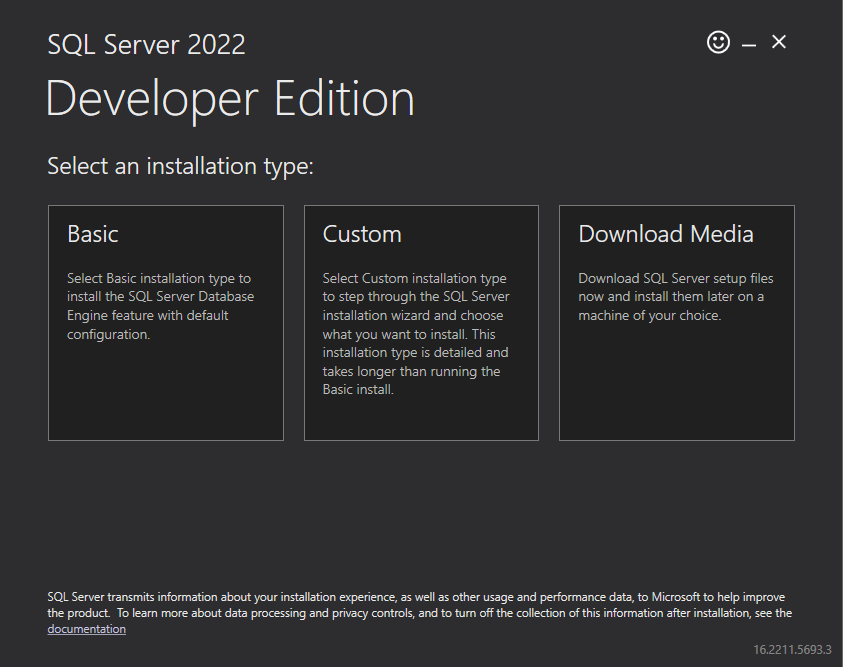
\includegraphics{./Figs/install2.png}
\end{frame}

\begin{frame}{Instaloni SQL Server}
\phantomsection\label{instaloni-sql-server}
\textbf{Hapi 2} Zgjidhni versionin
\end{frame}

\begin{frame}{Instaloni SQL Server}
\phantomsection\label{instaloni-sql-server-1}
Zgjidhni versionin bazë duke klikuar në opsionin ``Basic'', pasi ai ka
të gjithë konfigurimin e paracaktuar të kërkuar për të mësuar MS SQL.
\end{frame}

\begin{frame}{Instaloni SQL Server}
\phantomsection\label{instaloni-sql-server-2}
\textbf{Hapi 3} Pranoni kushtet

Do të shfaqet ekrani ``Kushtet e licencës së serverit të Microsoft''.
Lexoni Kushtet e Licencës dhe më pas klikoni ``Prano''.

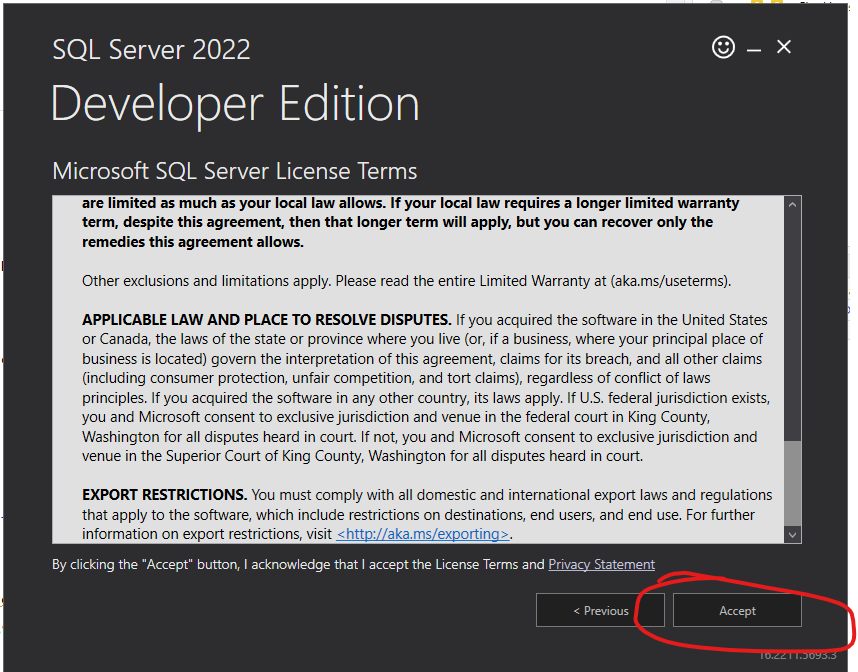
\includegraphics{./Figs/install3.png}
\end{frame}

\begin{frame}{Instaloni SQL Server}
\phantomsection\label{instaloni-sql-server-3}
\textbf{Hapi 4} Zgjidhni vendndodhjen

Më poshtë do të shfaqet dritarja ``Vendndodhja e instalimit të serverit
SQL'', e cila është një hap vendimtar në procesin e instalimit të
Microsoft SQL Server.
\end{frame}

\begin{frame}{Instaloni SQL Server}
\phantomsection\label{instaloni-sql-server-4}
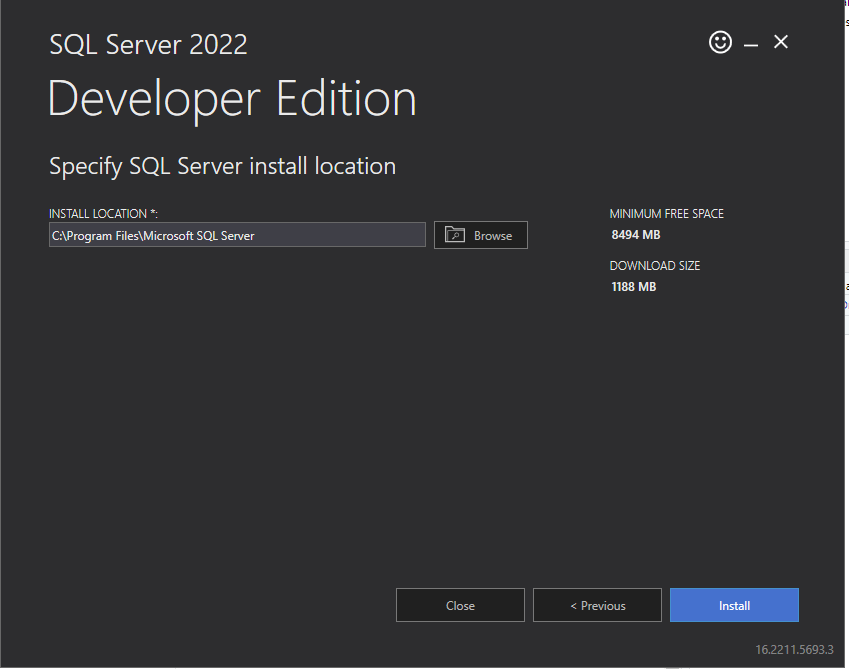
\includegraphics{./Figs/install4.png}

Vendndodhja e parazgjedhur është Program Files Microsoft SQL Server.
\end{frame}

\begin{frame}{Instaloni SQL Server}
\phantomsection\label{instaloni-sql-server-5}
\begin{itemize}
\item
  Opsionale, ne gjithashtu mund të ndryshojmë vendndodhjen e instalimit
  duke klikuar në \textbf{Browse}.
\item
  Pasi të zgjidhet vendndodhja, klikoni butonin ``Instalo'' për të
  filluar instalimin e SQL Windows 10.
\end{itemize}
\end{frame}

\begin{frame}{Instaloni SQL Server}
\phantomsection\label{instaloni-sql-server-6}
\begin{itemize}
\tightlist
\item
  Më poshtë do të shfaqet ekrani i progresit të ``Shkarkimit të paketës
  së instalimit''.
\end{itemize}

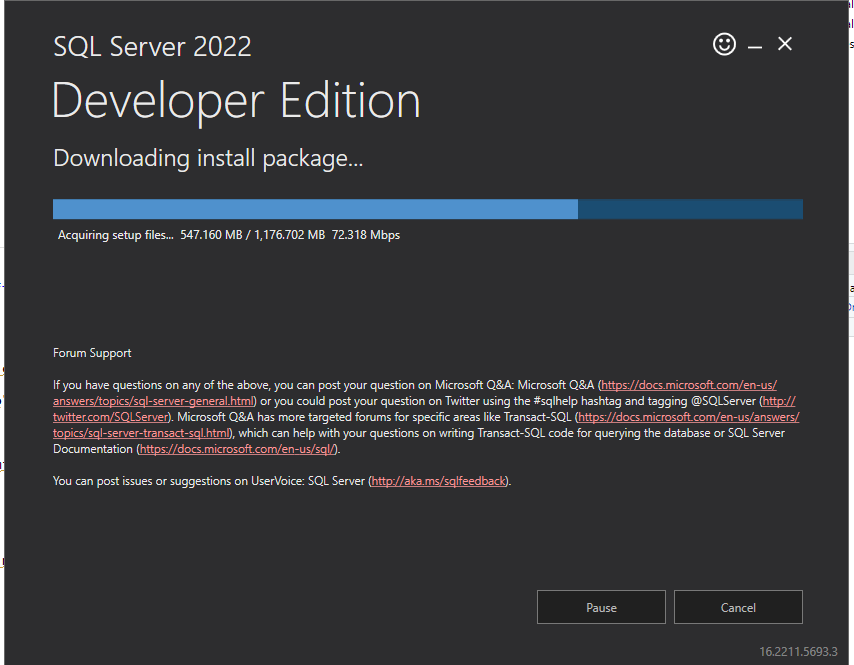
\includegraphics{./Figs/install5.png}

\begin{itemize}
\tightlist
\item
  Prisni derisa të përfundojë shkarkimi i softuerit SQL.
\end{itemize}
\end{frame}

\begin{frame}{Instaloni SQL Server}
\phantomsection\label{instaloni-sql-server-7}
Pasi shkarkimi të ketë përfunduar, sistemi do të fillojë instalimin e
versionit Developer.
\end{frame}

\begin{frame}{Instaloni SQL Server}
\phantomsection\label{instaloni-sql-server-8}
Më poshtë ekrani tregon përparimin e instalimit.

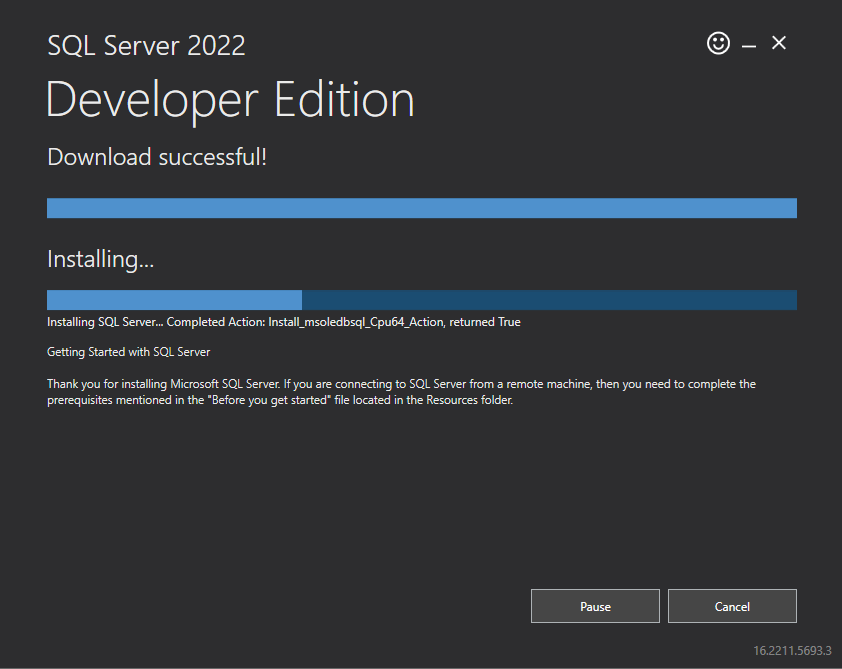
\includegraphics{./Figs/install6.png}
\end{frame}

\begin{frame}{Instaloni SQL Server}
\phantomsection\label{instaloni-sql-server-9}
\textbf{Hapi 5} Përfundoni procesin e instalimit

Pasi instalimi të përfundojë me sukses, do të shfaqet ekrani më poshtë.

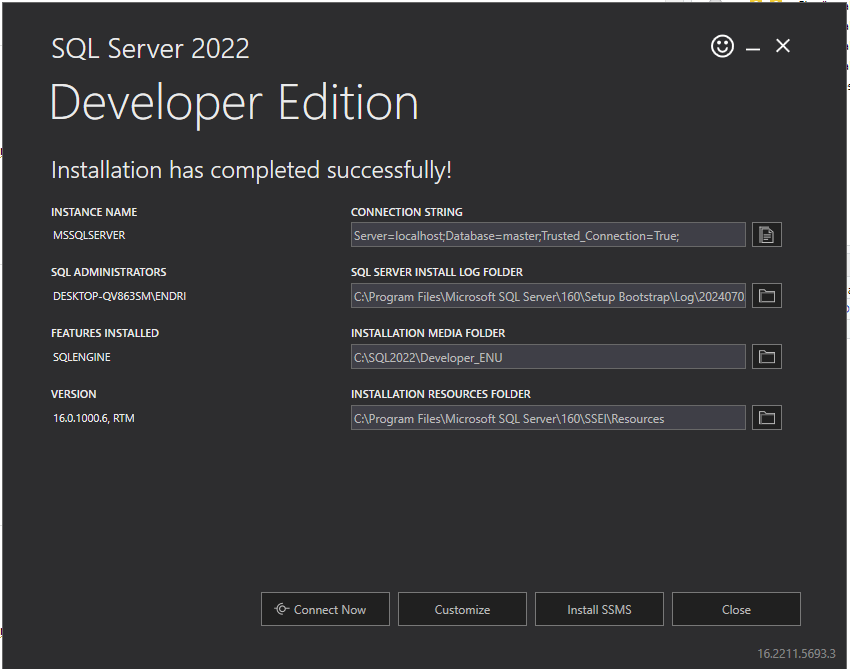
\includegraphics{./Figs/install7.png}
\end{frame}

\begin{frame}{Tani na duhet editor}
\phantomsection\label{tani-na-duhet-editor}
Hapim linkun :

\url{https://learn.microsoft.com/en-us/sql/ssms/download-sql-server-management-studio-ssms?view=sql-server-ver16\#download-ssms}
\end{frame}

\begin{frame}{Tani na duhet editor}
\phantomsection\label{tani-na-duhet-editor-1}
Shkarkojmë SQL Server Management Studio (SSMS) 20.1

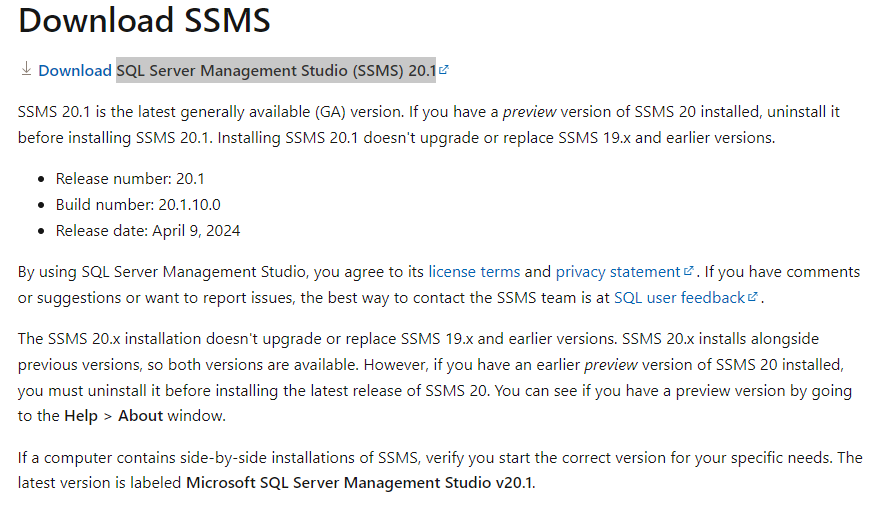
\includegraphics{./Figs/install8.png}
\end{frame}

\begin{frame}{Tani na duhet editor}
\phantomsection\label{tani-na-duhet-editor-2}
Instalojmë hap pas hapi
\end{frame}

\begin{frame}{Instaloni SQL Server}
\phantomsection\label{instaloni-sql-server-10}
Ky konfigurim është i vetë-mjaftueshëm për të vazhduar më tej me mësimin
e serverit SQL dhe ne mund ta `Mbyllim' këtë dritare.
\end{frame}

\section{Fillojmë}\label{fillojmuxeb}

\begin{frame}{Hyrje në SQL}
\phantomsection\label{hyrje-nuxeb-sql-1}
\begin{itemize}
\item
  SQL qëndron për \textbf{Structured Query Language} e cila përdoret për
  të punuar me bazat e të dhënave.
\item
  Serveri SQL dhe T-SQL (Transact-SQL) janë të dy RDMS (Sistemi i
  Menaxhimit të Bazave të të Dhënave Relacionale) ku ky i fundit ka
  funksione shtesë.
\end{itemize}
\end{frame}

\begin{frame}{Hyrje në SQL}
\phantomsection\label{hyrje-nuxeb-sql-2}
\begin{itemize}
\item
  SQL Server ruan të dhënat në formën e tabelave dhe lidhjeve.
\item
  Ne nuk mund të qasemi drejtpërdrejt në të gjitha të dhënat, kështu që
  përdorim pyetje \textbf{query} për të marrë të dhënat e duhura.
\end{itemize}
\end{frame}

\begin{frame}{Importimi i tabelës Excel në SQL}
\phantomsection\label{importimi-i-tabeluxebs-excel-nuxeb-sql}
\begin{itemize}
\item
  Hapim SQL Server Management Studio
\item
  Selectojmë majtas \textbf{Databases}
\end{itemize}
\end{frame}

\begin{frame}{Importimi i tabelës Excel në SQL}
\phantomsection\label{importimi-i-tabeluxebs-excel-nuxeb-sql-1}
\begin{itemize}
\tightlist
\item
  Me butonin e djathtë zgjedhim \textbf{New Database}
\end{itemize}

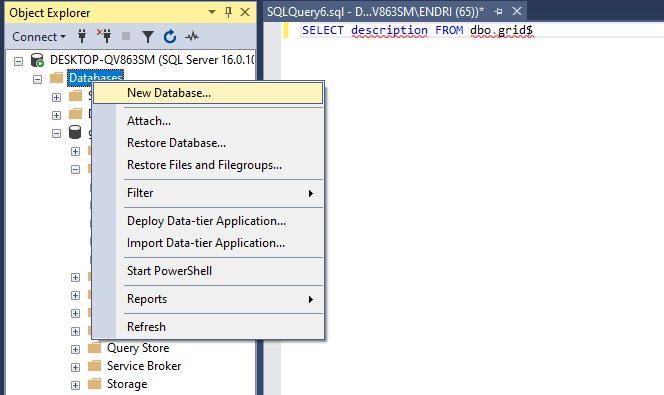
\includegraphics{./Figs/db1.png}
\end{frame}

\begin{frame}{Importimi i tabelës Excel në SQL}
\phantomsection\label{importimi-i-tabeluxebs-excel-nuxeb-sql-2}
\begin{itemize}
\tightlist
\item
  Te faqja e hapur vendosim emrin e databazës \textbf{grid} dhe OK
\end{itemize}

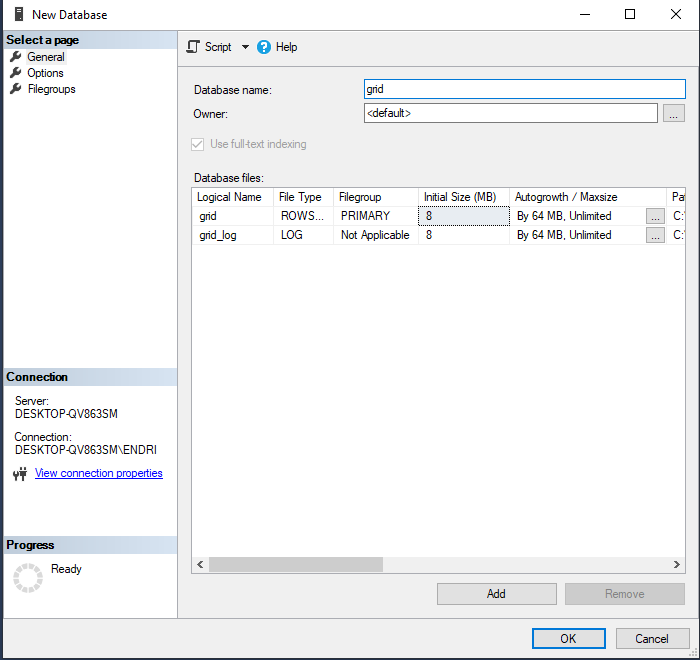
\includegraphics{./Figs/db3.png}
\end{frame}

\begin{frame}{Importimi i tabelës Excel në SQL}
\phantomsection\label{importimi-i-tabeluxebs-excel-nuxeb-sql-3}
\begin{itemize}
\tightlist
\item
  Te databaza e krijuar \textbf{grid} zgjedhim me butonin e djathtë
  Tasks - Import Data
\end{itemize}

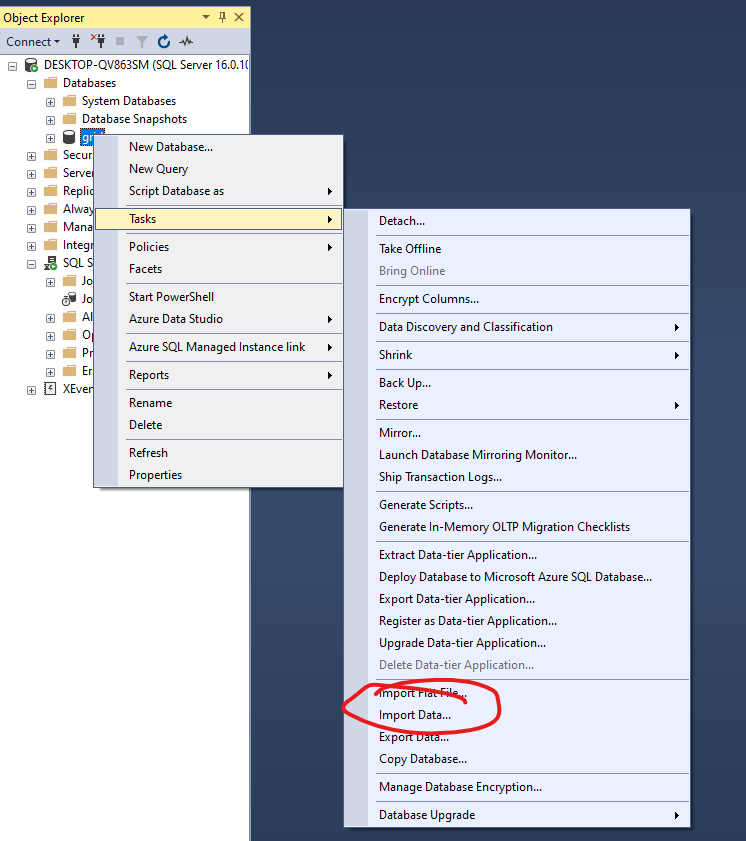
\includegraphics{./Figs/db4.png}
\end{frame}

\begin{frame}{Importimi i tabelës Excel në SQL}
\phantomsection\label{importimi-i-tabeluxebs-excel-nuxeb-sql-4}
\begin{itemize}
\tightlist
\item
  Navigojmë në folder ku kemi skedarin Excel \textbf{grid}
\end{itemize}

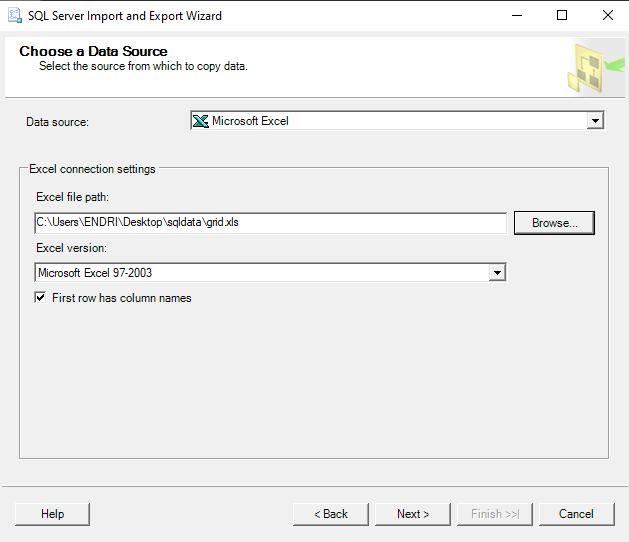
\includegraphics{./Figs/db5.png}
\end{frame}

\begin{frame}{Importimi i tabelës Excel në SQL}
\phantomsection\label{importimi-i-tabeluxebs-excel-nuxeb-sql-5}
\begin{itemize}
\tightlist
\item
  Në menunë e destinacionit zgjedhim \textbf{Microsoft Ole Db Provider
  for SQL Server}
\end{itemize}

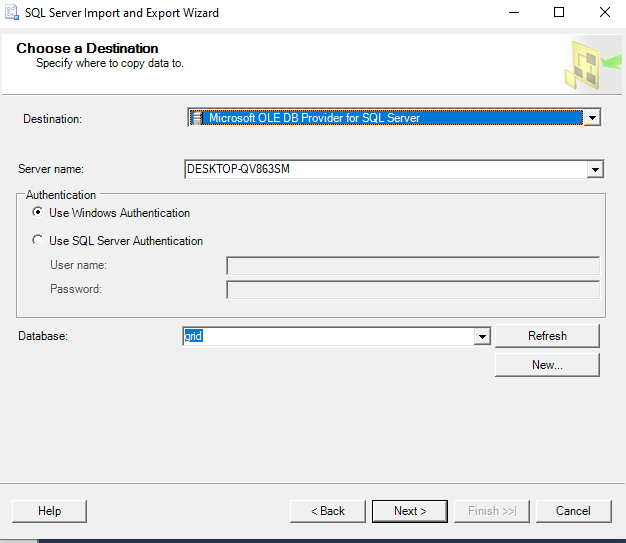
\includegraphics{./Figs/db6.png}
\end{frame}

\begin{frame}{Importimi i tabelës Excel në SQL}
\phantomsection\label{importimi-i-tabeluxebs-excel-nuxeb-sql-6}
\begin{itemize}
\tightlist
\item
  Në dritaret e tjera zgjedhim Next dhe Finish
\end{itemize}
\end{frame}

\begin{frame}{Importimi i tabelës Excel në SQL}
\phantomsection\label{importimi-i-tabeluxebs-excel-nuxeb-sql-7}
\begin{itemize}
\tightlist
\item
  Në qoftë se procesi ka shkuar OK do shfaqet tabela si në figurë
\end{itemize}

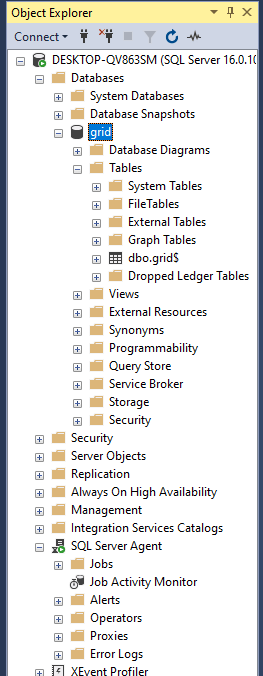
\includegraphics{./Figs/db8.png}
\end{frame}

\begin{frame}{Hyrje në SQL}
\phantomsection\label{hyrje-nuxeb-sql-3}
\begin{itemize}
\item
  Deklarata \textbf{SELECT} specifikon atë që duam të marrim nga tabela.
\item
  \textbf{FROM} specifikon vendndodhjen e tabelës burimore.
\end{itemize}
\end{frame}

\begin{frame}{Hyrje në SQL}
\phantomsection\label{hyrje-nuxeb-sql-4}
Gjithmonë përfundoni një pyetje me një \textbf{;}.
\end{frame}

\begin{frame}[fragile]{Shembull}
\phantomsection\label{shembull}
\begin{Shaded}
\begin{Highlighting}[]
\KeywordTok{SELECT}\NormalTok{ description }
\KeywordTok{FROM}\NormalTok{ dbo.grid$}
\end{Highlighting}
\end{Shaded}
\end{frame}

\begin{frame}{Shembull}
\phantomsection\label{shembull-1}
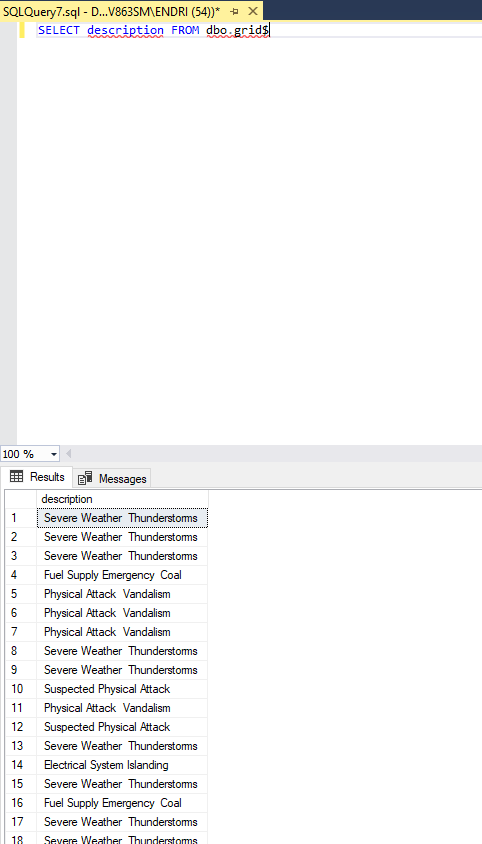
\includegraphics{./Figs/query1.png} \#\# Hyrje në SQL

\begin{itemize}
\item
  Përdorni \textbf{TOP} për të kufizuar numrin e rreshtave të kthyer.
\item
  Ne gjithashtu mund të specifikojmë përqindjen e rreshtave duke
  përdorur \textbf{TOP (5) PERCENT}.
\end{itemize}
\end{frame}

\begin{frame}[fragile]{Shembull}
\phantomsection\label{shembull-2}
\begin{Shaded}
\begin{Highlighting}[]
\KeywordTok{SELECT}\NormalTok{ TOP (}\DecValTok{5}\NormalTok{) }\KeywordTok{PERCENT}\NormalTok{ description}
\KeywordTok{FROM}\NormalTok{ dbo.grid$}
\end{Highlighting}
\end{Shaded}
\end{frame}

\begin{frame}{Shembull}
\phantomsection\label{shembull-3}
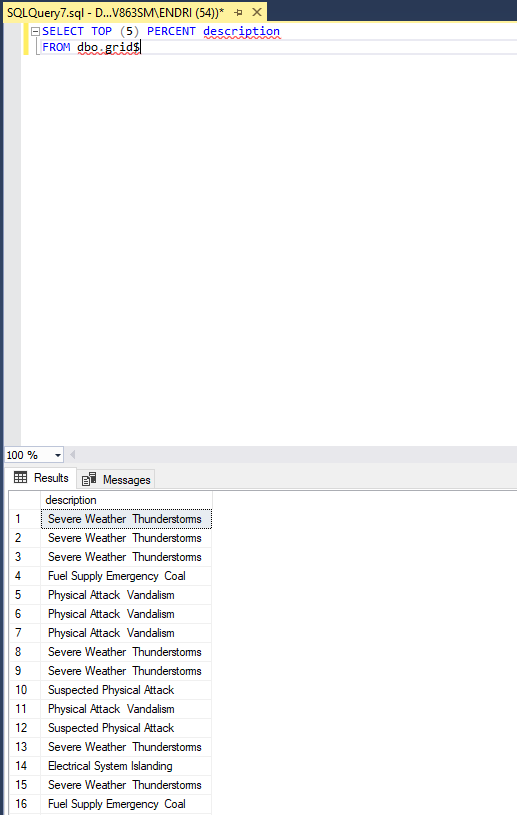
\includegraphics{./Figs/query2.png}
\end{frame}

\begin{frame}{Hyrje në SQL}
\phantomsection\label{hyrje-nuxeb-sql-5}
\begin{itemize}
\tightlist
\item
  Përdorni SELECT DISTINCT për të kthyer një listë me vlera unike nga
  një kolonë.
\end{itemize}
\end{frame}

\begin{frame}[fragile]{Shembull}
\phantomsection\label{shembull-4}
\begin{Shaded}
\begin{Highlighting}[]
\KeywordTok{SELECT}
  \KeywordTok{DISTINCT}\NormalTok{ country }\KeywordTok{AS}\NormalTok{ unique\_country}
\KeywordTok{FROM}
\NormalTok{  dbo.eurovis$;}
\end{Highlighting}
\end{Shaded}
\end{frame}

\begin{frame}{Shembull}
\phantomsection\label{shembull-5}
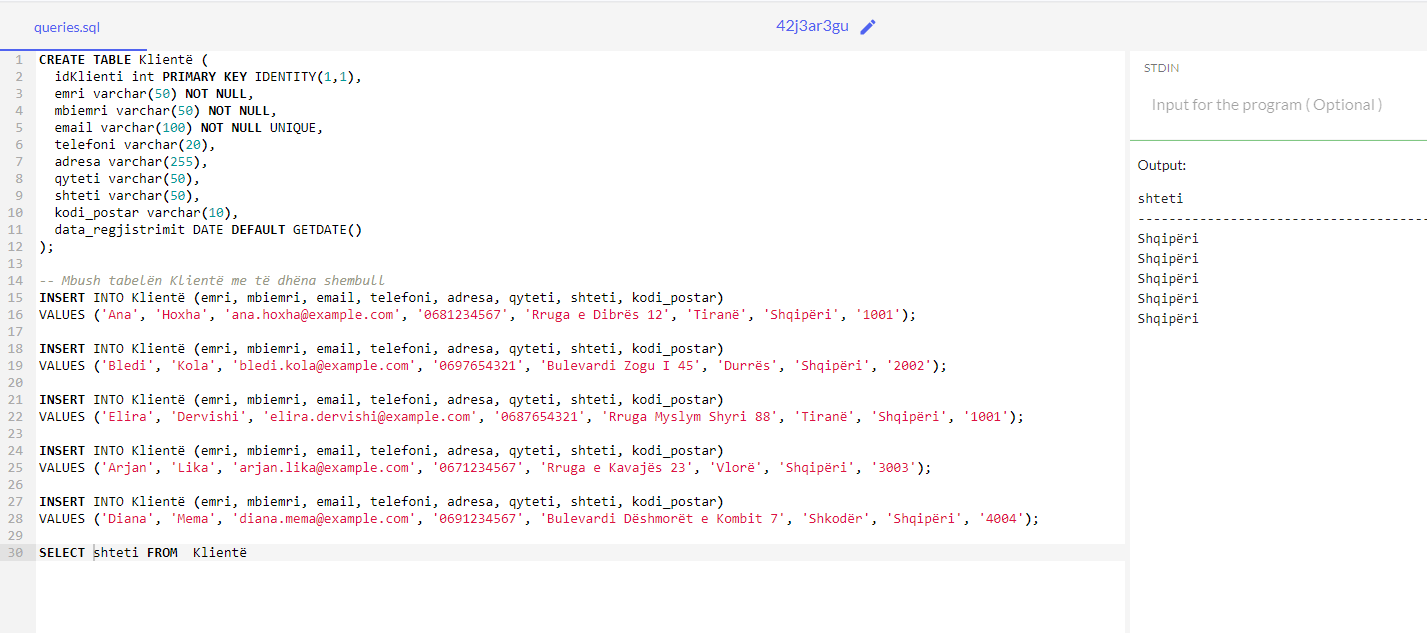
\includegraphics{./Figs/query4.png}\\
\#\# Hyrje në SQL

\begin{itemize}
\tightlist
\item
  Përdorni SELECT * për të kthyer të gjitha rreshtat e një kolone. (Nuk
  rekomandohet për tabela të mëdha).
\end{itemize}
\end{frame}

\begin{frame}[fragile]{Shembull}
\phantomsection\label{shembull-6}
\begin{Shaded}
\begin{Highlighting}[]
\KeywordTok{SELECT} \OperatorTok{*} \KeywordTok{FROM}
\NormalTok{  dbo.eurovis$;}
\end{Highlighting}
\end{Shaded}
\end{frame}

\begin{frame}{Shembull}
\phantomsection\label{shembull-7}
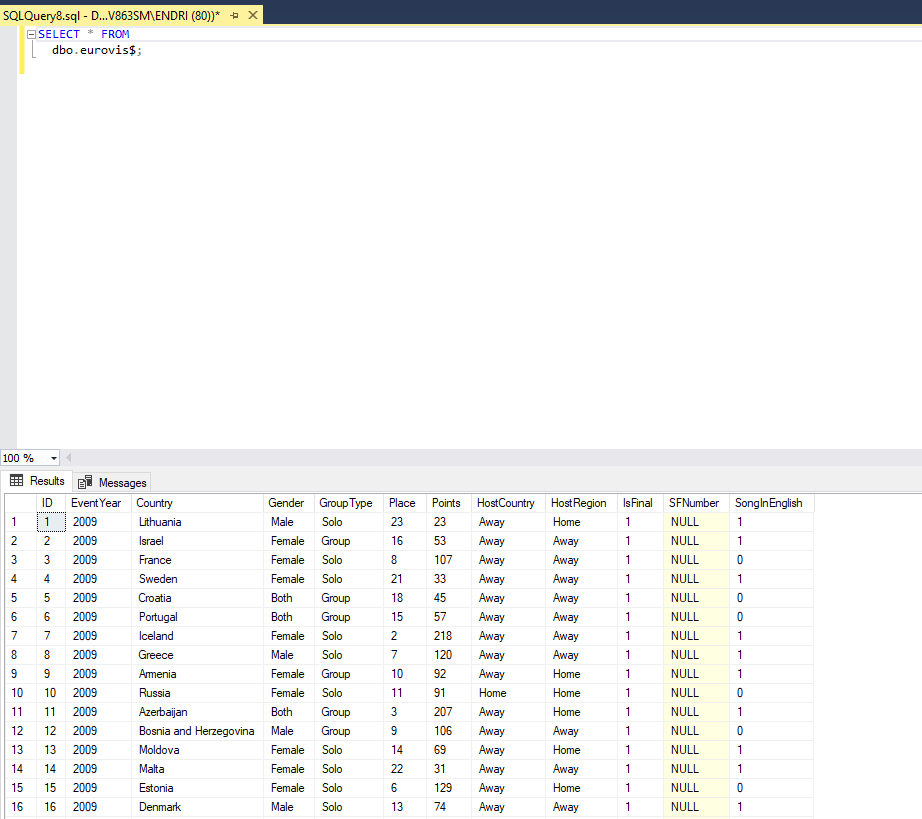
\includegraphics{./Figs/query5.png}
\end{frame}

\end{document}
